 %%
%%
\documentclass[12pt]{book}
\usepackage{amsfonts}
\usepackage{amsmath}
\usepackage{amssymb}
\usepackage{graphicx}
\usepackage{hyperref}
\usepackage{polynom}
\usepackage{amsthm}
\setlength{\textheight}{10in}
\setlength{\textwidth}{7.4in}
\setlength{\topmargin}{-0.75in}
\setlength{\oddsidemargin}{-0.5in}
\setlength{\evensidemargin}{-0.5in}
\setlength{\parskip}{0.15in}
\setlength{\parindent}{0in}

%commands
\newcommand\numberthis{\addtocounter{equation}{1}\tag{\theequation}}

\begin{document}


\vspace{-1.0in}\begin{center}
\Large{MHF4U : Advanced Functions }

\Large{Assignment \#2}


\end{center}

%\medskip

\vspace{0.015in}\hrulefill\ 

\textbf{Reference Declaration} %  Fill in your Reference Declarations in this section before your submit your assignment.

Complete the Reference Declaration section below in order for your assigment to be graded.

If you used any references beyond the course text and lectures (such as other texts, discussions with colleagues or online resources), indicate this information in the space below.  If you did not use any aids, state this in the space provided. 

Be sure to cite appropriate theorems throughout your work. You may use shorthand for well-known theorems like the FT (Factor Theorem), RRT (Rational Root Theorem), etc. 

Note: Your submitted work must be \textbf{your original work}. 

Family Name: Wong\\%Family Name Here
First Name: Max%First Name Here

Declared References: 

Used this forum answer to number the an element (Question 1): \\
\href{https://tex.stackexchange.com/questions/42726/align-but-show-one-equation-number-at-the-end}{stackexchange align* but show one equation number at the end} \\
Used YouTube tutorial to do long division with polynomials (Question 1 and 2): \\
\href{https://www.youtube.com/watch?v=9JfhV2Dimms} \\
Used Desmos for graphs

% Type your references here.
% You can use as many lines as required.

\vspace{0.015in}\hrulefill\ 

\newpage

%%%%%%%%%%%% PROBLEMS START HERE

\begin{enumerate}

%% PROBLEM 1
\item Given the volume of a rectangular box is $V(x) = x^3 + 6x^2 + 11x + 6$, if the length of the box is $x+3$ cm, and its width is $x+2$ cm then \textbf{determine} the height of the box. Also, \textbf{determine} the domain and range of the function $V$.

%% I would recommend sandwiching your solution to every problem between the kind of structure I have provided below re: initial \vspace, the Solution: heading and the ending \vspace.
%\vspace{0.3cm} 
%\textbf{Solution:}\\
% Your solution starts here.
%\vspace{0.3cm}

\vspace{0.3cm} 
\textbf{Solution to Question 1:}\\

 Considering v(x) has a degree of 3. We are also given the length and width, $x+3$ and $x+2$ respectively. This means that:

 $$(x+3)(x+2)(x+a) = v(x)$$

 Where $a \in \mathbb{R}$. We know that there are 3 factors because of the degree. Since:

 \begin{align*}
    v(x) &= x^3+6x^2+11x+6 \\
    \\
    \therefore (x+3)(x+2)(x+a) &= x^3+6x^2+11x+6 && \text{Combining the previously listed equations} && \textbf{(1)}
 \end{align*}

 Dividing both sides by $(x+3)(x+2)$:

 \addtolength{\jot}{1em}
 \begin{align*}
    (x+3)(x+2)(x+a) &= x^3+6x^2+11x+6 \\
    (x+a) &= \frac{x^3+6x^2+11x+6}{(x+3)(x+2)} \\
    (x+a) &= \frac{x^3+6x^2+11x+6}{x^2+5x+6} && \text{Expanding denominator bracket} \\
 \end{align*}
 
 \vspace{-3.5em}
 \begin{center}
     Now, using long division, find the final missing value factor, $(x+a)$:
 \end{center}
 \vspace{-2em}

%Do long division
$$\polylongdiv{x^3+6x^2+11x+6}{x^2+5x+6}$$

    $$\boxed{\therefore \text{the height of the box is x+1}}$$
    \vspace{1cm}
    \begin{center}
        Second part of solution on next page
    \end{center}
    \newpage

    Also since this relationship is of degree 3, it is a cubic function. Cubic functions have should 
    the properties of a domain and range of all real whole numbers but since the dimensions of a 
    of a 3D shape (Domain) cannot be negative in reality, the domain can only be 
    equal to or greater than zero. When the domain is at zero, or f(0), we can calculate the 
    minimum range value. 

    $$f(0) = 0^3+6\times 0^2+11\times 0+6 = 6$$
   
    $$\boxed{\therefore D: \{ x \in \mathbb{R} | x \geq 0 \} , R: \{ y \in \mathbb{R} | y \geq 6 \}}$$

\vspace{1cm}
\textbf{Check work for question 1 by graphing and using a logical check:}
\vspace{1em}
From before, we stated that $(x+3)(x+2)(x+a) = x^3+6x^2+11x+6$. Now that we know the value of a (1), redo the operation to check the work.

%Do Math Here
\begin{align*}
    x^3+6x^2+11x+6 &= (x+3)(x+2)(x+a)&& \text{From (1)}\\
    x^3+6x^2+11x+6 &= (x+3)(x+2)(x+1) && a = 1\\
    &= (x^2+5x+6)(x+1) && \text{multiply first 2 factors and simplify} \\
    &= x^3+6x^2+11x+6 && \text{expand and simplify}\\
    LHS &= RHS && \therefore \text{height is correct}
\end{align*}

\vspace{1em}
From the graph, we can also see that domain and range are all real whole numbers.

%Graph here
\vspace{1.5em}
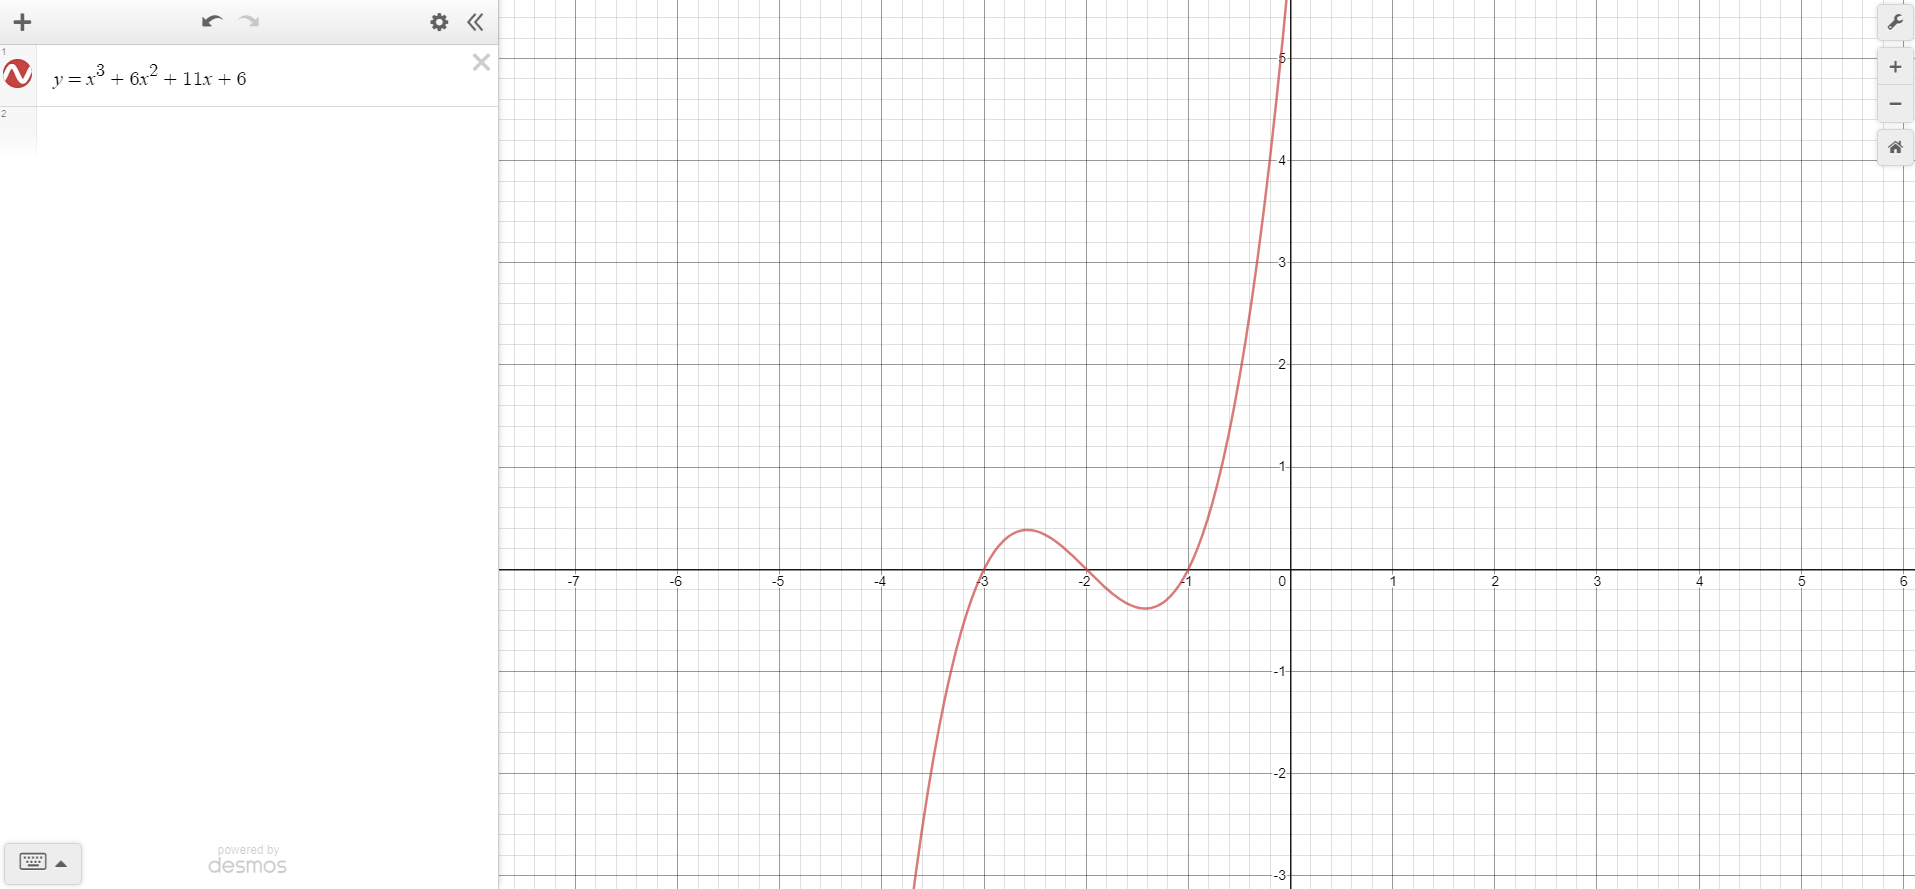
\includegraphics[width=\linewidth]{a2-1 graph.PNG}

\newpage

%% PROBLEM 2
\item Consider the quartic polynomial function $f(x) = x^4 - 5x^3 + x^2 + 21x - 18$. Given that there is a local minimum on $f(x)$ at $(-1,-32)$, use a logical argument to \textbf{prove} that this must be the absolute minimum of $f(x)$ without graphing the function. \\

Recall that $x=c$, where $c \in \mathbb{R}$, corresponds to a \emph{local minimum} of a function $f(x)$ on an interval $I = (a,b)$ which contains $c$ provided that for every value of $x$ on the interval $I$ we have that $f(c) \le f(x)$.

\vspace{0.3cm} 
\textbf{Solution for question 2:}\\
\begin{proof}
 If we can create a sign table from this function we can better visualize 
 the relaitonship and better prove the local minimum. First factor f(x) by 
 finding the values of x where f(x) = 0. We know that factors are typically between
 -6 and 6. From the Rational Root Theorum we can also narrow down our search by using
 factors of the last term divided by the factors of the first term, plus minus. Possible 
 candidates include x= -6, -3, -2, -1, 1, 2, 3 adnd 6.From experimentations:

 \vspace{-0.8cm}
 \begin{align*}
    f(1) &= 0 \\
    f(3) &= 0 \\
    f(-2) &= 0
 \end{align*}

To find the 4th missing factor, divide f(x) by the current 3 known factors found:

\begin{align*}
    \text{missing factor} &= \frac{x^4 - 5x^3 + x^2 + 21x - 18}{(x-1)(x-3)(x+2)} \\
    &= \frac{x^4 - 5x^3 + x^2 + 21x - 18}{(x^2-4x+3)(x+2)} && \text{expand and simplify denominator}\\
    &= \frac{x^4 - 5x^3 + x^2 + 21x - 18}{(x^3+2x^2-4x^2-8x+3x+6} \\
    &= \frac{x^4 - 5x^3 + x^2 + 21x - 18}{(x^3-2x^2-5x+6} && \text{simplified}
\end{align*}

\vspace{0.2cm}
\begin{center}
    Now use long division
\end{center}
\vspace{-0.5cm}
$$\polylongdiv{x^4 - 5x^3 + x^2 + 21x - 18}{x^3-2x^2-5x+6}$$

\newpage

$\therefore$ in factor form $f(x) = {(x-3)}^2(x-1)(x+2)$. Since f(x) is positive 
(no negative vertical reflection) and utilizing the x intercepts given by the factor form:

\begin{center}
    \begin{tabular}{|c|c|c|c|c|}
        \hline
        & ($-\infty$, -2) & (-2, 1) & (1, 3) & (3, $\infty$) \\ \hline
        x + 2 & $-$ & + & + & + \\ \hline
        x - 1 & - & - & + & + \\ \hline
        x - 3 & - & - & - & + \\ \hline
        x - 3 & - & - & - & + \\ \hline
        f(x) & + & - & + & + \\ \hline
    \end{tabular}
\end{center}

Using the intervals from the sign table above and the known propterties 
of linear and quadratic factors, we can create a rough diagram:

%diagram here
\begin{center}
    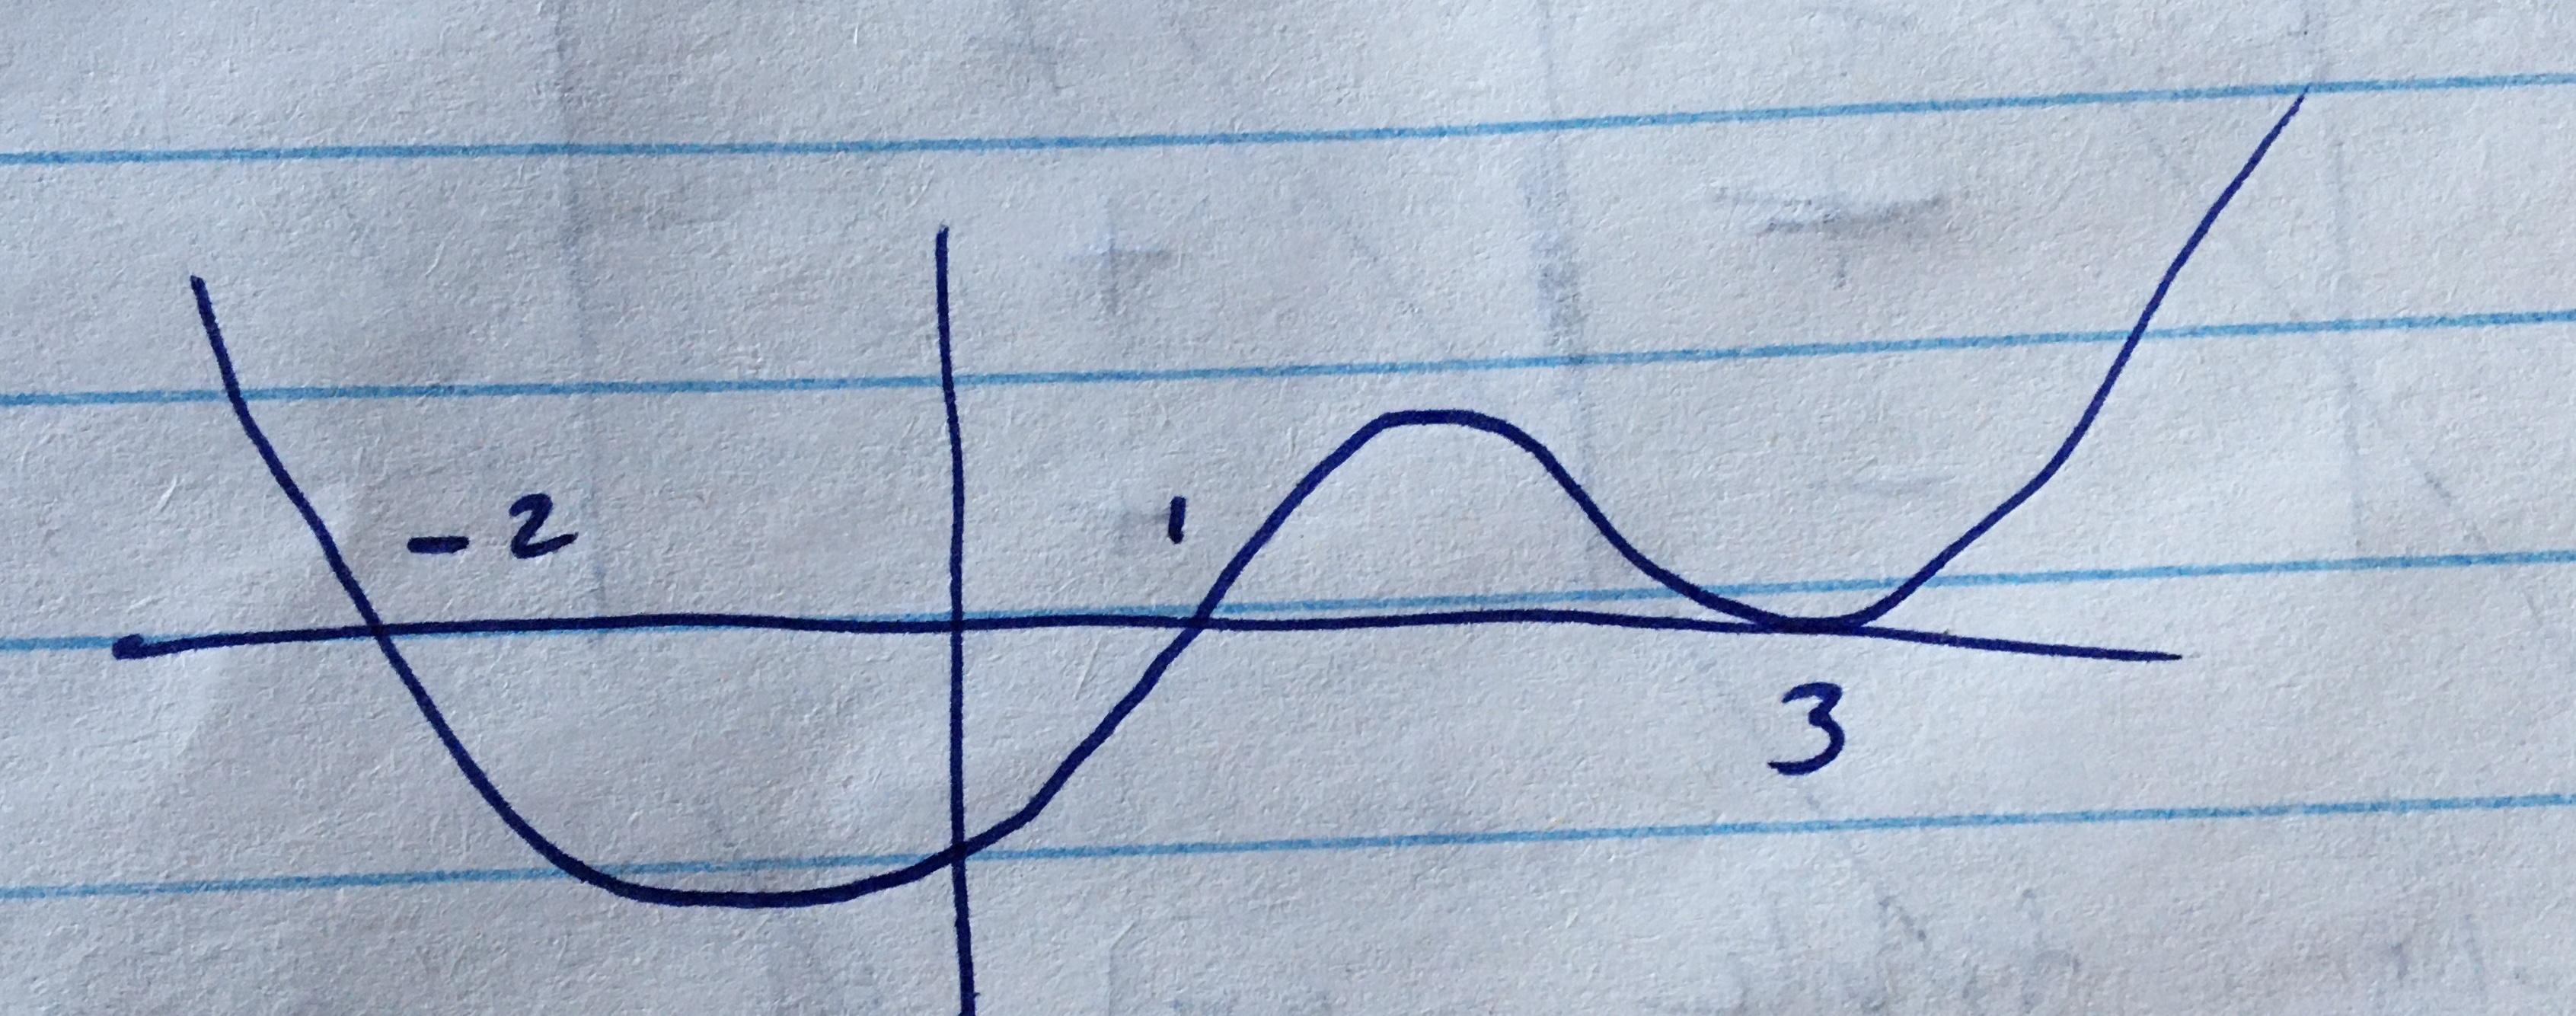
\includegraphics[scale=0.06]{A2-2 Diagram.jpeg}
\end{center}

\vspace{0.5cm}
We can agree that the minimum points have the lowest values, and theoretically 
with a positive quadric function there are two possible negative areas where the minimum
is likely to reside within (since the negative interval sections are the lowest points). 
On the diagram these spots are the areas where rate of change goes from negative to 
positive (angled down proceeded by an angle up).

\vspace{1cm}
\fbox{\parbox{\textwidth}{Lets check these two candidates. One of the possible minimums, where x=3, the line "skims"
the x-axis. This means that this segment does not actually drop into the negative parts 
of the cartesian plane. This means that the only area that goes negative, at interval (-2, 1),
is where the local minimum must reside. Since the x value x=-1 of the coordinate (-1, -32) is inside
the previously identified interval, we can conclude that this coordinate is likely the local minimum. \qedhere}}
\end{proof}

\vspace{2cm}
\begin{center}
    Proof is on the next page
\end{center}

\newpage

\vspace{0.5cm}
\textbf{Prove question 2 answer with a secondary proof using derivatives:}
\vspace{0.3cm}

If we factor the derivative of the function, the factors will produce the 
x values for the points of relative extreme value.

\begin{align*}
    f(x) &= x^4 - 5x^3 + x^2 + 21x - 18 \\
    f'(x) &= 4x^{4-1} - 5 \times 3x^{3-1} + 2x^{2-1} + 21x^{1-1} && \text{Get the derivative}\\
    f'(x) &= 4x^3 - 15x^2 + 2x^1 + 21 && \text{simplify} \\
\end{align*}

Now factor the derivative: From experimentation we can find that:

\begin{align*}
    f'(-1) &= 0 \\
    f'(3) &= 0 \\
    f'\left( \frac{7}{4} \right) &= 0
\end{align*}

Therefore these are the points of extreme values, the only places where a 
local minimum and maximum are possible. Now, if we find the f(x) value of these numbers
 we can determine their y values.

 \begin{align*}
    f(-1) &=  -33\\
    f(3) &=  0\\
    f\left( \frac{7}{4} \right) &\approx 4.395 
\end{align*}

From this we can see that (-1, -33) is the lowest value.
 $\therefore$ this proves that (-1, -33) is indeed the local extreme value.

\vspace{0.3cm}

\newpage

%% PROBLEM 3
\item Recall that a prime number is defined as an integer $n>1$ such that its only positive divisors are 1 and $n$. Let $\mathbb{P}$ represent the set of prime numbers. Suppose that you know that when you divide $g(x) = x^3 + 2x^2 + cx + d$ by $x-2$ you obtain a remainder of 14, \textbf{determine} the specific values of $c$ and $d$ given that $c \in \mathbb{Z}$ and $d \in \mathbb{P}$. 

\vspace{0.3cm} 
\textbf{Solution to question 3:}
\vspace{0.5 cm}
 Since we know that $g(x)$ divided by $x-2$ gives a remainder of 14,
 We can compare try the division and compare the resulting polynomial remainder
with the real value of 14. Since we know a factor is ax $x=2$ (from $x-2$) leads 
to a remainder or y value of 14, we can state that $g(2) = 14$.

\begin{align*}
    g(x) &= x^3 + 2x^2 + cx + d \\
    g(2) &= 2^3 + 2\times 2^2 + c\times 2 + d && \text{Substitute x as 2}\\
    g(2) &= 8 + 8 + 2c + d && \text{Simplify}\\
    g(2) &= 16 + 2c + d \\
    14 &= 16 + 2c + d && g(2) = 14\\
    -2 &= 2c + d && \text{Subtract 16 from both sides}\\
\end{align*}

\vspace{-1cm}

Now that we have the equation $-2 = 2c + d$ and we know that $d \in \mathbb{P}$ and $c \in \mathbb{Z}$, consider the following.

In the equation $-2 = 2c + d$, c is multiplied by 2. This means 
that no matter the value of c, if it is an integer, the value 
of 2c must be even. 2c and d are added together to also create 
an even number: -2. When are two numbers are added together to 
an even number both numbers must be even or both must be odd. 
This means if 2c is even, d must also be even. The only prime 
number that exists is 2 since all other numbers that are even 
are divisible by 2. Therefore d must be 2. From this and the 
equation, we can determine the value of c.

\vspace{-0.6cm}

\begin{align*}
    -2 &= 2c + d \\
    -2 &= 2c + 2 && \text{Substitute d as 2} \\
    -2 - 2 &= 2c && \text{subtract 2 to both sides}\\
    -4 &= 2c && \text{Simplify} \\
    \frac{-4}{2} &= c && \text{divide both sides by 2} \\
    -2 &= c
\end{align*}

$$\boxed{\therefore \text{the value of c and d are -2 and 2 respectively.}}$$

\newpage

\textbf{Check Answer for Question 3 by substituting the know values of c and d back into the original equation as g(2) = 14:}

\begin{proof}
    \begin{align*}
        g(x) &= x^3 + 2x^2 + cx + d && \text{Original equation}\\
        g(x) &= x^3 + 2x^2 - 2x + 2 && \text{Since }c = -2, d = 2\\
        g(2) &= 2^3 + 2\times 2^2 - 2\times 2 + 2 && \text{Substitute x as 2}\\
        14 &= 2^3 + 2\times 2^2 - 2\times 2 + 2 && g(2) = 14\\
        14 &= 8 + 8 - 4 + 2\\
        14 &= 14 \\
        LHS &= RHS && \qedhere\\
    \end{align*}
\end{proof}

\vspace{-1cm}
$$\therefore \text{the values of c and d found are correct}$$

\newpage

%% PROBLEM 4
\item Solve $\dfrac{7}{x+2} + \dfrac{5}{x-2} = \dfrac{10x-2}{x^2 - 4}$.

\vspace{0.5cm} 
\textbf{Solution to question 4:}

\vspace{0.3cm} 
To solve isolate all values to one side of the equal sign before simplifying. Then, when fully simplified, take the numerator and solve for x.

\begin{align*}
    \dfrac{7}{x+2} + \dfrac{5}{x-2} &= \dfrac{10x-2}{x^2 - 4} \\
    \dfrac{7}{x+2} + \dfrac{5}{x-2} - \dfrac{10x-2}{x^2 - 4} &= 0 && \text{subtract } \dfrac{10x-2}{x^2 - 4} \text{ from both sides}\\
    \dfrac{7}{x+2} + \dfrac{5}{x-2} - \dfrac{10x-2}{(x+2)(x-2))} &= 0 && x^2-4 = (x+2)(x-2)\\
    \dfrac{7(x-2)}{(x+2)(x-2)} + \dfrac{5(x+2)}{(x-2)(x+2)} - \dfrac{10x-2}{(x+2)(x-2))} &= 0 && \text{Get common denominators} \\
    \dfrac{7(x-2)+5(x+2)-(10x-2)}{(x+2)(x-2)} &= 0 && \text{Add all fractions together}\\
    \dfrac{7x-14+5x+10-10x+2}{(x+2)(x-2)} &= 0 && \text{Expand and Simplify}\\
    \dfrac{2x-2}{(x+2)(x-2)} &= 0\\
\end{align*}

\vspace{-0.8cm} 
Now take the numerator and solve for x:
\vspace{-0.2cm} 

\begin{align*}
    \dfrac{2x-2}{(x+2)(x-2)} &= 0\\
    2x-2 &= 0\\
    2x &= 2 && \text{subtract 2 from both sides}\\
    \therefore x &= 1 && \text{divide all by 2}\\
\end{align*}

\vspace{-1cm} 
$$\boxed{\therefore \text{the solution to } \dfrac{7}{x+2} + \dfrac{5}{x-2} = \dfrac{10x-2}{x^2 - 4} \text{ is } x = 1}$$

\vspace{1cm} 
\begin{center}
    Proof is on next page
\end{center}

\newpage
\textbf{prove question 4 by substituting x=1 back into the original equation:}\\

%proof goes here
\begin{proof}
    \begin{align*}
        LHS &= \dfrac{7}{x+2} + \dfrac{5}{x-2} \\
        &= \dfrac{7}{1+2} + \dfrac{5}{1-2} && \text{Substitute x as 1} \\
        &= \dfrac{7}{3} + \dfrac{5}{-1} && \text{Simplify} \\
        &= \dfrac{7}{3} + \dfrac{-15}{3} \\
        LHS &= -\dfrac{8}{3}
    \end{align*}

    \begin{align*}
        RHS &= \dfrac{10x-2}{x^2 - 4} \\
        &= \dfrac{10\times 1-2}{1^2 - 4} && \text{Substitute x as 1} \\
        &= \dfrac{10-2}{1 - 4} && \text{Simplify}\\
        RHS &= -\dfrac{8}{3}\\
        RHS & =LHS && \qedhere
    \end{align*}
\end{proof}

$\therefore$ the answer is correct. 

\newpage

%% PROBLEM 5
\item Solve $\bigg|\dfrac{x-4}{x+5}\bigg| \le 4$.

\vspace{0.3cm} 
\textbf{Solution to question 5:}

\vspace{0.5cm}
 Consider the following identity of an absolute value inequality: $|x| \leq c \Longleftrightarrow -c \leq x \leq c$
 . Lets apply this to the given equation where c is 4 and x is the absolute value rational function.
 \vspace{-0.3cm}

 \begin{align*}
    \bigg|\dfrac{x-4}{x+5}\bigg| &\le 4 \\
    -4 \le \dfrac{x-4}{x+5} & \le 4 && \text{applying identity}
 \end{align*}

Now solve the inequality found as if it were composed of two seperate inequalities with the rational function being repeated twice:

\begin{align*}
    -4 &\le \dfrac{x-4}{x+5} && (1)\\
    \dfrac{x-4}{x+5} &\le 4 && (2)
\end{align*}

\vspace{1cm}

%Solving (1)
Take (1), $-4 \le \dfrac{x-4}{x+5}$ and solve the inequality.

\begin{align*}
    -4 &\le \dfrac{x-4}{x+5} && (1)\\
    0 &\le \dfrac{x-4}{x+5} + 4 && \text{add 4 to both sides} \\
    0 &\le \dfrac{x-4}{x+5} + \dfrac{(4)(x+5)}{x+5} && \text{Get same denominator} \\
    0 &\le \dfrac{x-4}{x+5} + \dfrac{(4x+20}{x+5} && \text{Expand} \\
    0 &\le \dfrac{x-4+4x+20}{x+5} && \text{Add fractions} \\
    0 &\le \dfrac{5x+16}{x+5} && \text{Simplify} \\
\end{align*}

\newpage

\begin{center}
To solve the rational inequality, we create a sign table
 to determine the appropriate intervals.
\end{center}
\vspace{0.5cm}

\begin{center}
    \begin{tabular}{|r|c|c|c|}
        \hline
        & $(-\infty, -5)$ & $\left(-5, -\dfrac{16}{5} \right)$ & $\left( -\dfrac{16}{5}, \infty \right)$ \\ \hline
        5x+16 & - & - & + \\ \hline
        x+5 & - & + & + \\ \hline
        f(x) & + & - & + \\ \hline
    \end{tabular}
\end{center}

\vspace{0.3cm}

Since we are searching for values greater than or equal to zero,
 look for the intervals where the value is positiive or zero. We can see
  from the sign table that, when including the values at zero:

$$x \in (-\infty, -5], \left[ -\frac{16}{5}, \infty \right) \text{\space\space\space\space\space} (3)$$

\vspace{1cm}

%Solving (2)
Take (2), $\dfrac{x-4}{x+5} \le 4$ and solve the inequality.

\begin{align*}
    \dfrac{x-4}{x+5} &\le 4 && (2)\\
    \dfrac{x-4}{x+5} - 4 &\le 0 && \text{subtract 4 to both sides} \\
    \dfrac{x-4}{x+5} - \dfrac{(4)(x+5)}{x+5} &\le 0 && \text{Get same denominator} \\
    \dfrac{x-4}{x+5} - \dfrac{4x+20}{x+5} &\le 0 && \text{Expand} \\
    \dfrac{x-4-(4x+20)}{x+5} &\le 0 && \text{Combibe fractions} \\
    \dfrac{x-4-4x-20}{x+5} &\le 0 && \text{expand} \\
    \dfrac{-3x-24}{x+5} &\le 0 && \text{Simplify} \\
    \dfrac{3x+24}{x+5} &\geq 0 && \text{Multiply by -1 to all, flip inequality sign} \\
\end{align*}

\newpage

\begin{center}
To solve the rational inequality, we create a sign table
 to determine the appropriate intervals.
\end{center}
\vspace{0.5cm}

\begin{center}
    \begin{tabular}{|r|c|c|c|}
        \hline
        & $(-\infty, -8)$ & $(-8, -5)$ & $(-5, \infty)$ \\ \hline
        3x+24 & - & + & + \\ \hline
        x+5 & - & - & + \\ \hline
        f(x) & + & - & + \\ \hline
    \end{tabular}
\end{center}

\vspace{0.3cm}

Since we are searching for values greater than or equal to zero,
 look for the intervals where the value is positiive or zero. We can see
  from the sign table that, when including the values at zero:

$$x \in (-\infty, -8], [-5, \infty) \text{\space\space\space\space\space} (4)$$
\vspace{0.1cm}

Now let's combine the intervals found from (1) and (2). We can do this by 
plotting the intervals on a line diagram and look for the intervals where
(3) and (4) overlap. In essence we need to find intervals that satisfy both 
inequalities, which is why we look for overlap.

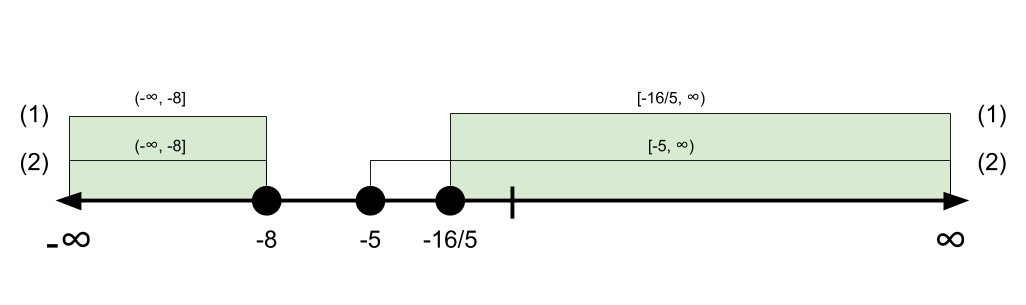
\includegraphics[width=\linewidth]{A2-5 Line Diagram (1).png}

From the line diagram, we can see that the 4 intervals overlap at 2 areas,
 highlighted by the green.
 
$$\boxed{\therefore \text{the intervals that satisfy the inequality} \bigg|\dfrac{x-4}{x+5}\bigg| \le 4 \text{ are } (-\infty , -8] \cup \left[ -\dfrac{16}{5}, \infty \right) \text{.}}$$

\vspace{2cm}
\begin{center}
    Proof is on the next page
\end{center}

\newpage

\textbf{Prove the intervals found in question 5 with a graph:}

\begin{center}
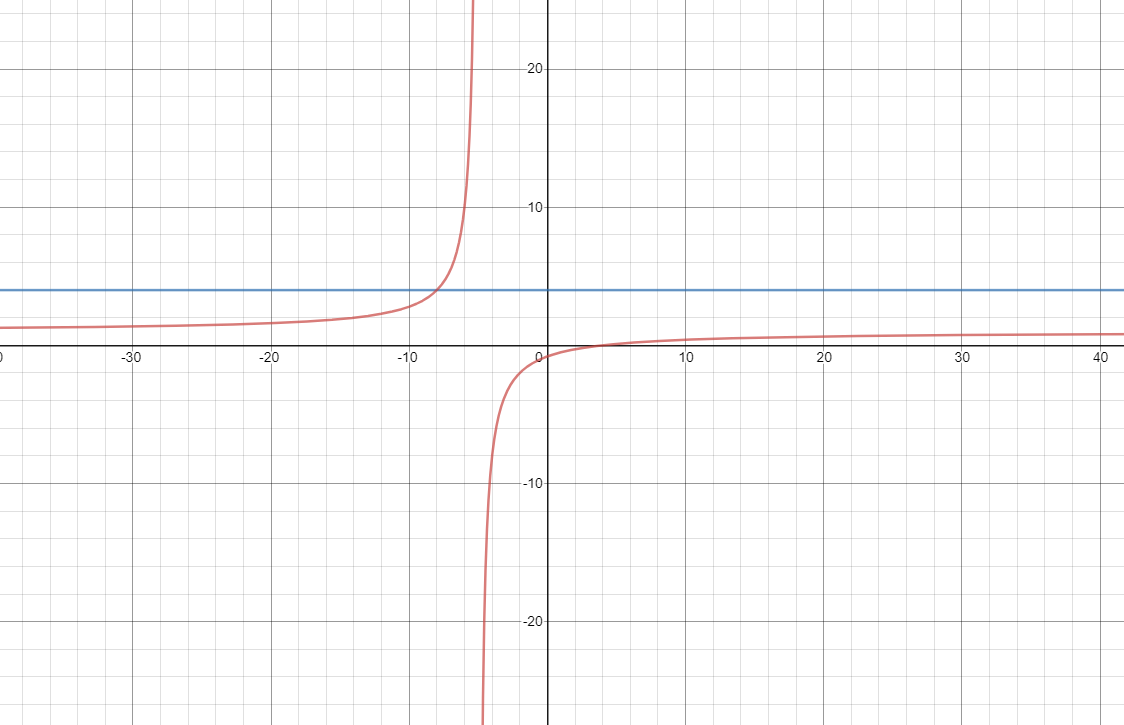
\includegraphics[scale = 0.7]{A2-5 Proof.PNG}
\end{center}

\vspace{0.5cm}
From the graph we can see that the intervals found seem to intervals
 on the graph that exist below or equal to y=4.

\newpage

\end{enumerate}

\end{document} 
